\documentclass[a4paper]{article}
\input{packages}
\title{Information and knowledge managment final project }
\author{Mateusz Grotek, Jože Kraner}
\date{}
\begin{document}
\maketitle
\begin{abstract}
The report describes ''eXpertIze'' program, which is a knowledge application software, for helping users to realize what they have in mind, fulfilling some constraints. It could be used both as a game, which allows to guess the name of an object a player has in mind by asking him/her some questions, and as a serious software module for discovering what a user has in mind when e.g. learning a language, and not remembering a word. The algorithm used is general. We focused on the game functionality.
\end{abstract}
\tableofcontents
\section{Introduction}
Let us consider the general knowledge discovery problem. The process of knowledge discovery was defined in \citet{Memon} as ''the development of new tacit or explicit knowledge from data and information or from the synthesis of prior knowledge''. Depending if an individual wants to gain explicit or tacit knowledge, possible strategies are combination of knowledge and socialization. 

Let us imagine the following situation: a user does not remember a word in a foreign language. He or she knows exactly what he or she wants to say. A knowledge discovery system could help him or her to find a proper word describing an object he or she has in mind by utilizing what he or she already knows about the thing. The same strategy could be used for the knowledge capturing process, which was defined in \citet{Memon} as ''the process of retrieving either explicit or tacit knowledge that resides within people, artifacts or organizational entities''. The difference between the two situations is the difference between the place the knowledge goes, it could be either a person or a knowledge base. In the knowledge discovery situation a person wants to gain some new knowledge. In the knowledge base situation an organization wants to transfer some knowledge from people's minds to organization's knowledge base. The source of the possibility of using the same algorithm lies in the following observation: in the presented situation a person is the source of knowledge. Nevertheless the end user of knowledge is different.

To be able to solve the problem we need to specify it further and to simplify it. The reasons for that are both time constraints and perceived difficulty of fully solving the problem. For this reason, we imagined the following scenario. A user has a material object in mind (but not \textbf{necessarily} a name of the object). By the least number of interactions with the user and by using a proper knowledge base we should be able to guess a name of the object. 
\section{Literature review}
There are two general ways of solving the problem. The first question we should as is: ''who should drive the interaction?''. The possibilities are the following: interaction should be driven ether by a user, or by a system. For user driven interaction there are many possible algorithms. The problem is very similar to the web searching problem. Let us imagine the following situation. A user has an object in mind, but he or she does not remember the name of it. By using some related queries to a web search engine he or she is possible to find a name of the object. For a way to implement this solution please consult \citet{Google}.

We decided to use the other way, which is driving interaction by the system. In this case it is the system who asks question to a user. By using this method our system is more general and we could pose the problem as a game between a user and the system. It means, that our algorithm could be used in entertainment. Because of that our problems transforms to a problem the very similar problem of 20 questions game. 20 questions was a popular american radio program airing from 1946 to 1954 (for more information consult: \citet{Radio}), but the game is based on a popular game ''Animal, vegetable or mineral?''. The problem of 20 questions game is as follows. A user has an object in mind. By asking him or her 20 questions to which he or she can answer only ''yes'', ''no'' or ''cannot tell'' we have to guess a name of the object. The only difference is the limitation to yes/no/cannot tell answers. Because each question can be transformed to a set of questions of the yes/no type the solution is not less general, but the number of questions can be much larger. We decided to pose our problem as a 20 questions game. 

As far as 20 questions problem existing algorithmic solutions are concerned the most comercially successful one is the solution patented by \citet{20Q} and used in a popular electronic device called 20Q. The algorithm used there is an artificial neural network. It maps the set of possible question/answer pairs to the set of possible objects. The main advantage of this system is a possibility of learning: the system asks a user if the answer is correct and changes the weights in neural network accordingly. The main disadvantage of the system is impossibility of influencing choices made by a system by changing knowledge base of the system. The knowledge is hidden in neuron weights and is not easily accessible for selective modification.

We decided to use a different method of solving the problem. We used Prolog programming language for implementing a knowledge base and a system operating over it. Prolog is a general purpose logic programming language used in many domains, especially in artificial intelligence and computational linguistics. It was created by \citet{Prolog} and implements a subset of first order logic called horn clauses, with a method of reasoning called SLD-resolution invented by \citet{SLD}. For more information about prolog please consult \citet{Prolog1}, \citet{Prolog2}, \citet{Prolog2}. As a logic programming language prolog have many advantages when creating artificial intelligence and computational linguistics programs. One of them is that it is very easy to implement reasoning in prolog programs. Another one is the database operations can be coded inside the language, and transparent database can be part of a program. These characteristics made Prolog very popular tool for creating logical reasoning programs, expert systems and other types of rule based systems. The addition of definite clause grammars to the syntax of Prolog allowed it to be used as an efficient tool in natural language processing systems. Despite the reputation of logic and rule based systems as beeing unable to implement fuzziness it is actually quite simple to do that in prolog. Because of these and other features of Prolog we decided to use it to create our system. Although \citet{20Q} states that: ''another major problem that is readily apparent in such systems is their incapability to handle inaccurate or misleading information if a player answers one question inaccurately this will cause the system to pursue the wrong branch of the decision tree leading it to the wrong answer or guess'', it was very easy to overcome this difficulty by implementing specific ''soft'' rule of reasoning. What we gained is a clear and easy to modify structure of the knowledge base, which was absent in the system based on neural networks.
\section{System architecture}
\subsection{Engine}

\subsection{Knowledge base}
%Database part - Joze. Mateusz - Engine
When we were designing our system, we decided that it will consist out of two parts - engine and knowledge base. In this section the knowledge base will be described in more detail.

Why do we need a knowledge base? The system is asking questions, and this questions must be stored somewhere. But, if this knowledge base would store only questions, it would be called a database. So, our knowledge base store more than just questions.

\begin{itemize}
\item  \textbf{Relations} - Each of this relations stored in knowledge base is representing a question about the object in mind. We can say that each question about the object is representing one attribute of an object. Here is an example of one relation named \verb|can_put_in_backpack.1.pl|.

\begin{lstlisting}[caption=Relation can\_put\_in\_backpack.1.pl,label=lst:relationexample]

question_about('Can all variations of it be put in a backpack?',can_put_in_backpack).
possibility_reduction(0.3,can_put_in_backpack).
can_put_in_backpack(X) :- can_put_in_pocket(X).
\end{lstlisting}

In this relation are stored: the question about the attribute ( \verb|'Can all variations of it be put in a backpack?'|), name of the attribute (\verb|can_put_in_backpack|), and a possibility reduction value(\verb|0.3|). The possibility reduction value is always defined as a value between 0 an 1, and represents how good, or how bad is the question. This question 'Can all variations of it be put in a backpack' is not very good, because if for example a user have in mind a projector, he might answer with yes. But the question was called 'Can \textbf{all variations} of it be putted into a backpack', so the answer should be no, because there are big cinema projectors, which can not be putted into a backpack. Problem is because not all users would think of these big projectors, so they will answer in a wrong way. Because we want to avoid the influence of users making mistakes in answering the questions, we set this possibility reduction value. This value 0.3 means, that if user answers with no, engine will 'add 0.3 to all the objects that have this attribute. And when object have this value more than 1, the engine stops asking questions about this object. So, it is good if bad questions have possibility reduction value less than 0.5 and good questions, such as ('Is it an animal?') should have possibility reduction value more than 0.5. With this value, we allow a user to make mistakes when answering the questions.
In relation \verb|can_put_in_backpack.1.pl|. there is also, line '\verb|can_put_in_backpack(X) :- can_put_in_pocket(X).|'. This means that if something can be putted into a pocket, than it also can be putted into a backpack. This enables the engine advanced reasoning. 


\item \textbf{Objects} - Our knowledge base, consist only of few objects. We created small but complete base of objects. But the aim was not to create a big database, but to create a good system, so the knowledge base could be expanded in future. Here is an example of an object in the knowledge base.
\begin{lstlisting}[caption=Object book.pl,label=lst:objectexample]
can_put_in_backpack(book).
can_be_opened_closed(book).
consist_of_pages(book).
\end{lstlisting}
Each object that is stored, includes the information about the names of the attributes this object has.
\end{itemize}

We created a simple window application called \textbf{Knowledge base manager}, for work with objects and attributes. The application is very simple and it just represent an idea in which direction this system could be developed.

    \begin{figure}[h]
      \begin{center}
		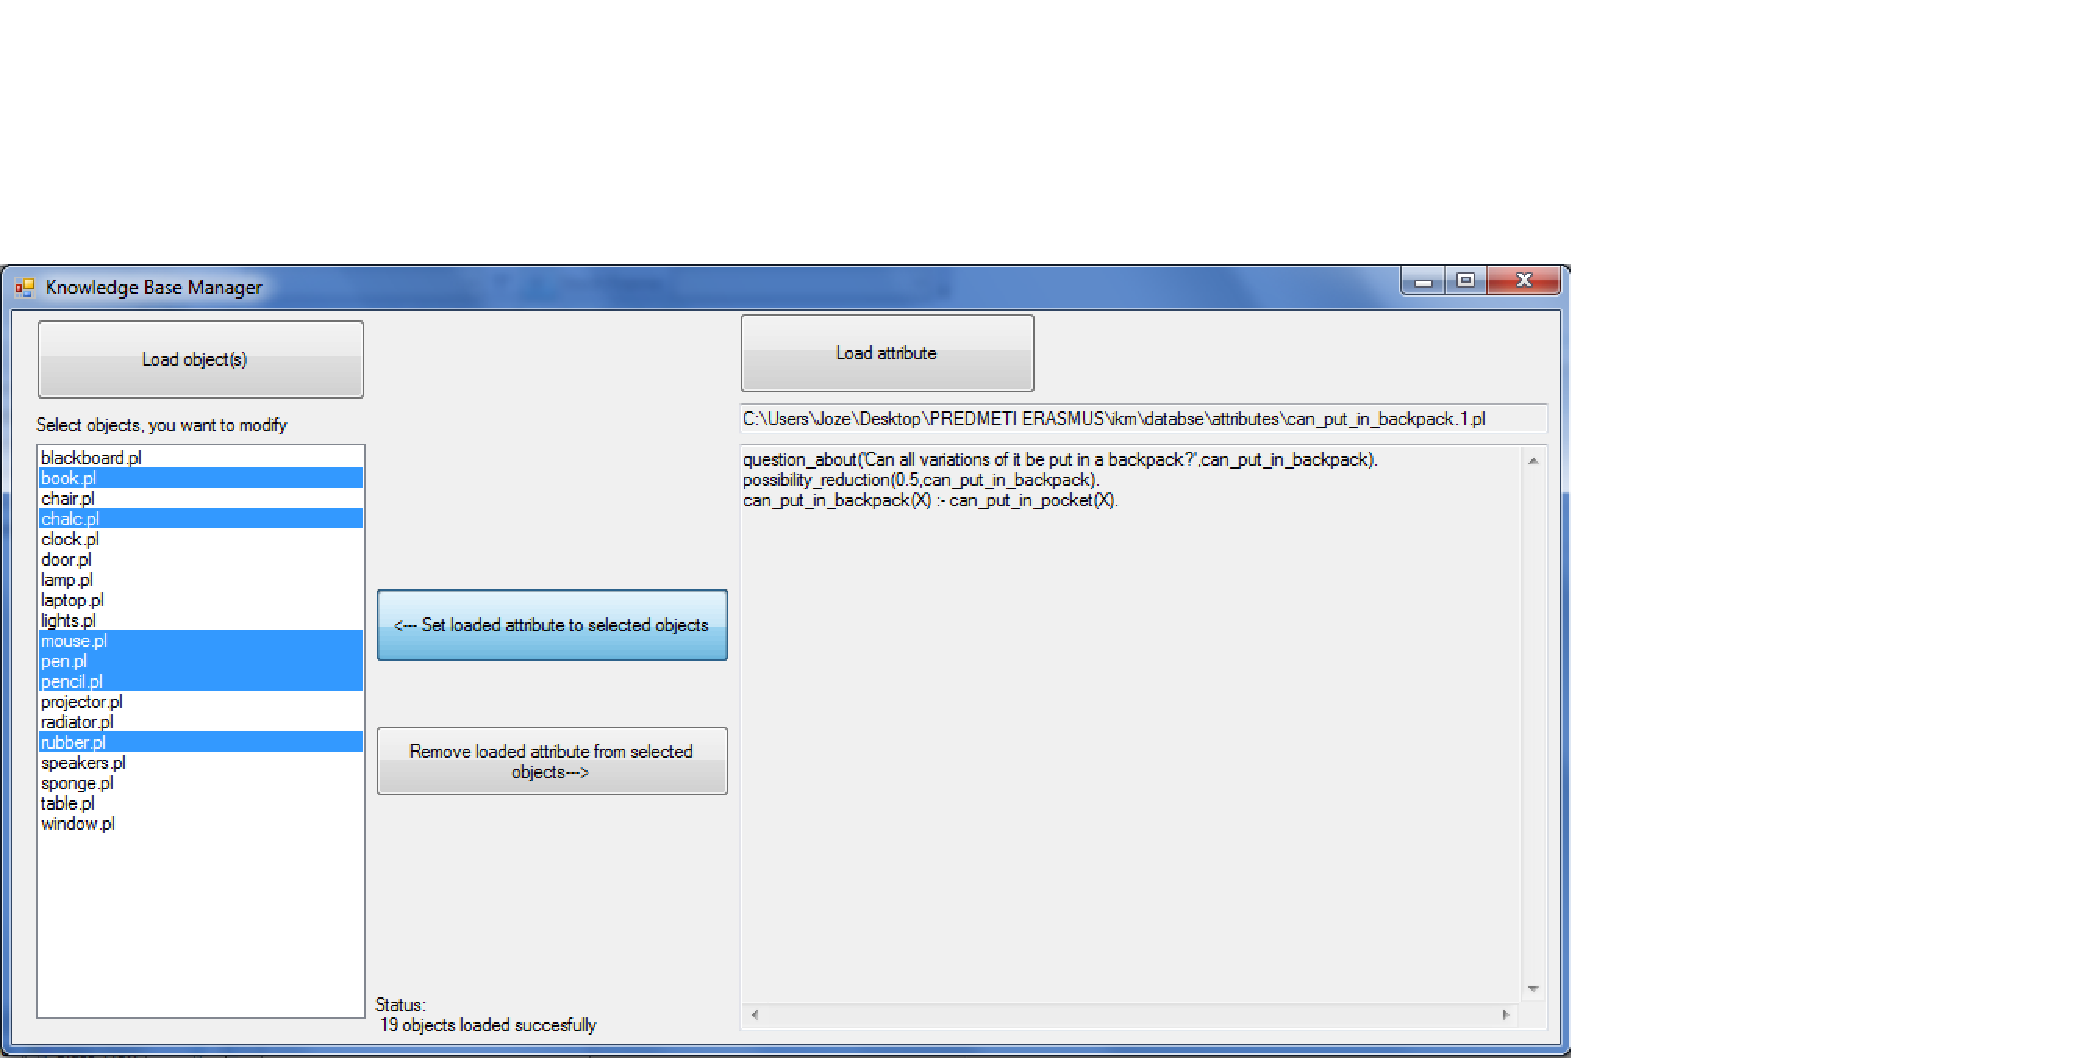
\includegraphics[scale=0.55]{img/KnowledgeBaseManagerPicture.png}	
\caption{Knowledge base manager application
\label{fig:SearchOptions}}
      \end{center}
    \end{figure}
    
As showed in the figure, this application allows object manipulation, which is, assigning attributes to the objects or removing attributes from the objects.


How to build a good knowledge base? There is an article about 20 question game \citet{howToAskQuestions} that helped us build the knowledge base. Here we found some good advices, for example which questions should be asked at the beginning. An example of an very bad question is 'Is it big?'. This is bad question because it is a question of degree, when it should be a question of comparison. So better question is 'Is it bigger than a backpack'.

\section{Limitations}
%Joze
As said before, the usage of this system is general. It could be used for entertainment or as an some other tool. One limitation this system has is the knowledge base. For now, the objects and relations (attributes) must be putted in manually. Second limitation is that the  objects are not learned about their attributes by our system, but the attributes must be assigned manually. Another limitation is that, a user could not answer the question only with 'yes' or 'no'. So there is no multiple possible answers such as 'I do not know' and so on.
 
\section{Conclusions and future work}
% Joze
There is a lot of things in domain of this system that could be improved. Here is some suggestions.

\begin{itemize}
\item \textbf{Filling the knowledge base} - The knowledge base could be filled automatically, using information found on the internet. For example, it could use wikipedia to learn about objects and their attributes. That is how the knowledge base could be expanded. Application 'Knowledge base manager' that was created could be improved. 

\item \textbf{More answers} - We could offer a user more different possible answers to the question. For example 'I do not want to answer'. This feature would reduce mistakes that users make when they are forced in 'yes or no' answers.

\item \textbf{Different questions} - The development of this feature is probably more complex, but it would be useful. System could be upgraded in a way, that it would ask questions like 'If you could describe an object with one word, what it would be?'. So the system could connect the answer with the object user have in mind.

Without doubt, the system that was developed has a lot of potential. The algorithm of choosing questions can be used in much more bigger knowledge base. So the future work should be focused in the expansion of the knowledge base. 

\end{itemize}
%The following references are just examples.
\begin{thebibliography}{10}
\bibitem[Memon(2011)]{Memon}Memon, N. 2011. \textsl{Information and Knowledge Management} --- lecture notes. University of Southern Denmark, Odense. \url{http://www.mip.sdu.dk/~memon/IKM_2011.htm}
\bibitem[Brin \& Page(1998)]{Google} Brin, S. and Page, L. 1998. \textsl{The Anatomy of a Large-Scale Hypertextual Web Search Engine.} In: Seventh International World-Wide Web Conference, 1998. Brisbane, Australia.
\bibitem[Van Deventer family(1946)]{Radio}Twenty Questions --- radio program. \url{http://www.otrcat.com/twenty-questions-p-1948.html}
\bibitem[Burgener(2005)]{20Q}Burgener R. 2005. \textsl{Artificial Neural Network Guessing Method and Game.} United States Patent Application Publication, Pub. No.: 2006/0230008 A1, Appl. No. 11/102,105, 2006. United States. \url{http://www.google.com/patents?id=W5iZAAAAEBAJ}
\bibitem[XXX(2000)]{Prolog}XXX
\bibitem[XXX(2000)]{SLD}XXX
\bibitem[XXX(2000)]{Prolog1}XXX
\bibitem[XXX(2000)]{Prolog2}XXX
\bibitem[XXX(2000)]{Prolog3}XXX
\bibitem[Eivind Nilssen (2005)]{howToAskQuestions} Nilssen, E. 2005. The game of twenty questions. \url{http://barelybad.com/20_questions.htm}
%\bibitem[Bernacki i in.(2005)]{BWG}Bernacki, M., Włodarczyk, P., Gołda, A. 2005. \textsl{Principles of training multi-layer neural network using backpropagation.} Katedra Elektroniki AGH, Kraków. \url{http://galaxy.agh.edu.pl/~vlsi/AI/backp_t_en/backprop.html}
%\bibitem[Frank i Asuncion(2010)]{FA}Frank, A., Asuncion, A. 2010. \textsl{{UCI} Machine Learning Repository: Iris Data Set.} University of California, Irvine, School of Information and Computer Science. \url{http://archive.ics.uci.edu/ml/datasets/Iris}
%\bibitem[Rojas(1996)]{RR}Rojas, R. 1996. \textsl{Neural Networks --- A Systematic Introduction.} Springer-Verlag, Berlin.
%\bibitem[Rutkowski(2005)]{LR}Rutkowski, L. 2005. \textsl{Metody i techniki sztucznej inteligencji.} PWN, Warszawa.
\end{thebibliography}
\end{document}
